\subsection*{Logaritmo e Exponencial}
\begin{tcolorbox}
Se $x, y >0$,$a>0$ e $\neq 0$, então:
\begin{align*}
    &\log_ax =y  \iff a^y=x\\
    &\ln{x}=\log_e{x}, \quad \text{onde} \quad \ln{e}=1\\
    &\ln{x}=y \iff  e^y=x
\end{align*}
%$$$$
\begin{multicols}{2}
\subsubsection*{Propriedades: Logaritmo}
 $\log_{a}(xy)=\log_{a}x + \log_{a}y$\\[0.1cm]
 $\log_{a}(\frac{x}{y})=\log_{a}x  \log_{a}y$\\[0.1cm]
 $\log_{a}(x^y)=y\log_{a}x$\\[0.1cm]
$\log_{a}c=\frac{\log_{b}c}{\log_{b}a}$\\[0.1cm]
 $a^{\log_a x}=a$\\[0.1cm]
 $\log_aa^x =x$%\\[0.2cm]

 \subsubsection*{Gráficos}
 \begin{Figure}
     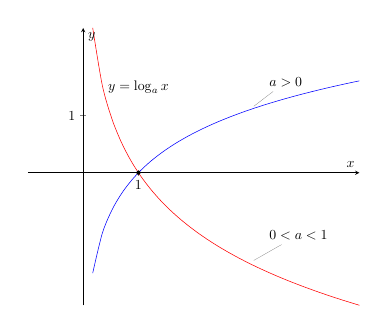
\begin{tikzpicture}[scale=0.5]
\begin{axis}[
 axis lines=middle,
 ticklabel style={fill=white},
xmin=-1.,%xmax=1.5,
%ymin=-1,ymax=5,
 xlabel=$x$,ylabel=$y$,
 domain=0:5,
 samples=30,
 smooth,
 xtick={1},ytick={1},
 yticklabels={1},   xticklabels={1},
 width=10cm]
\coordinate  (x2) at (1,e);
\coordinate  (x1) at (1,0);
\addplot[blue] {ln(x)};
\addplot[red] {(ln(x)/ln(0.5))};
\fill[black] (x2) circle (1.5pt);
\fill[black] (x1) circle (1.5pt);

\node[] at (axis cs:1,{1.5}) {$y=\log_a{x}$};

\node[pin= 50:{$a>0$}] at (axis cs:3,{ln(3)}) {};
\node[pin= 50:{$0<a<1$}] at (axis cs:3,{(ln(3)/ln(0.5)}) {};
\end{axis}
\end{tikzpicture}
 \end{Figure}
\end{multicols}
 \end{tcolorbox}
\begin{tcolorbox}

\begin{multicols}{2}
\subsubsection*{Propriedades: Exponencial}
 $a^{-x}=\dfrac{1}{a^x}$\\
 $(a^x)^y=a^{xy}$\\
 $a^xa^y=a^{x+y}$\\
 $(ab)^x=a^xb^x, \forall b>0$\\
 $a^0=1$\\
 se $a>1,x<y \implies a^x < a^y$ \\
 se $0<x<1\implies a^x> a^y$
 \subsubsection*{Gráficos}
 \begin{Figure}
     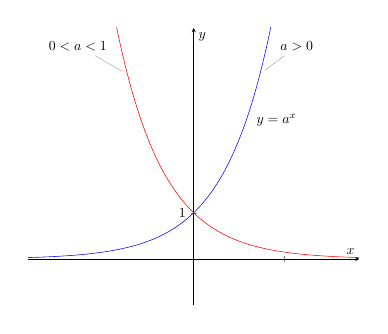
\begin{tikzpicture}[scale=0.5]
\begin{axis}[
 axis lines=middle,
 ticklabel style={fill=white},
xmin=-5.,%xmax=1.5,
ymin=-1,ymax=5,
 xlabel=$x$,ylabel=$y$,
 domain=-5:5,
 samples=30,
 smooth,
 xtick={2.7182},ytick={1},
 yticklabels={1},   xticklabels={,,},
 width=10cm]
\coordinate  (x2) at (e,1);
\coordinate  (x1) at (0,1);
\addplot[blue] {2^(x)};
\addplot[red] {(1/2)^x)};
% \fill[black] (x2) circle (1.5pt);
% \fill[black] (x1) circle (1.5pt);

%\draw[dashed] (x1)--(x2) --(e,0);
\node[] at (axis cs:2.5,{3}) {$y=a^{x}$};

\node[pin= 50:{$a>0$}] at (axis cs:2,{2^(2)}) {};
\node[pin= 130:{$0<a<1$}] at (axis cs:-2,{(1/2)^(-2)}) {};
\end{axis}
\end{tikzpicture}
 \end{Figure}
\end{multicols}
\end{tcolorbox}
